\documentclass[a4paper,10pt]{article}
\usepackage[utf8]{inputenc}
\usepackage[spanish]{babel}
\usepackage[affil-it]{authblk}
\usepackage{enumerate}
\usepackage{graphicx}
\usepackage{hyperref}
\usepackage{amsmath}
\usepackage{amssymb}
\usepackage{cancel}
\usepackage[usenames, dvipsnames]{color}
\usepackage{tikz}
\usepackage[labelfont=bf]{caption}
\usepackage{subcaption} %Multiple images
\usepackage{multicol} % Multiple columns
\usepackage{float}
\usepackage{cleveref}
 \usepackage{relsize} % bigger math symbols
\usepackage[margin=1.4in]{geometry}
\usepackage[titletoc,toc,title]{appendix}
\usepackage{enumitem}
\usetikzlibrary{calc}
\numberwithin{equation}{section}

%Appendices in spanish
\renewcommand{\appendixname}{Ap\'endices}
\renewcommand{\appendixtocname}{Ap\'endices}
\renewcommand{\appendixpagename}{Ap\'endices}

%Zero delimiter
\newcommand{\zerodel}{.\kern-\nulldelimiterspace}

%Columns separation
\setlength{\columnsep}{1cm}

%Indentation
\setlength{\parindent}{0ex}

%Multiple References

\crefrangelabelformat{equation}{(#3#1#4--#5\crefstripprefix{#1}{#2}#6)}

\usepackage{xparse}

%Boxes

\newcommand*{\boxcolor}{blue}
\makeatletter
\renewcommand{\boxed}[1]{\textcolor{\boxcolor}{%
\tikz[baseline={([yshift=-1ex]current bounding box.center)}] \node [rectangle, minimum width=1ex,rounded corners,draw] {\normalcolor\m@th$\displaystyle#1$};}}
 \makeatother

%Constantes
\newcommand{\euler}{\mathrm{e}}
\newcommand{\im}{i}

%Lemas, teoremas, definiciones y pruebas
\newcommand{\definicion}{\textbf{Definición: }}
\newcommand{\lema}{\textbf{Lema: }}
\newcommand{\teorema}{\textbf{Teorema: }}
\newcommand{\prueba}{\textbf{Prueba: }}
\newcommand{\proposicion}{\textbf{Proposición: }}
\newcommand{\corolario}{\textbf{Corolario: }}


%opening
\title{Mecánica Clásica Tarea \# 10}
\author{Favio Vázquez\thanks{Correo: favio.vazquezp@gmail.com}}\affil{Instituto de Ciencias Nucleares. Universidad Nacional Autónoma de México.}
\date{}

\begin{document}

\makeatletter
\def\@maketitle{%
  \newpage
  \null
  \vskip 2em%
  \begin{center}%
  \let \footnote \thanks
    {\Large\bfseries \@title \par}%
    \vskip 1.5em%
    {\normalsize
      \lineskip .5em%
      \begin{tabular}[t]{c}%
        \@author
      \end{tabular}\par}%
    \vskip 1em%
    {\normalsize \@date}%
  \end{center}%
  \par
  \vskip 1.5em}
\makeatother

\maketitle

\section{Problema 1}

Utilizando la formulación hamiltoniana de la mecánica, encuentre las ecuaciones de 
movimiento de un péndulo doble de masas y longitudes iguales.

\vspace{.3cm}

\underline{Solución:} \vspace{.3cm}

En la figura de abajo se muestra un diagrama para el problema,

\begin{figure}[H]
 \center
 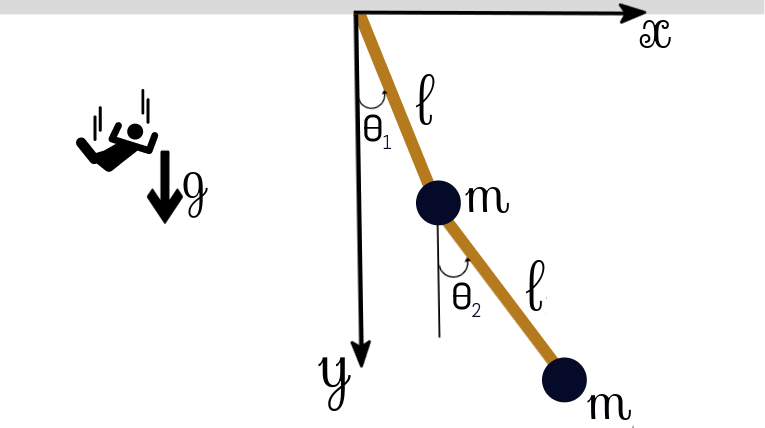
\includegraphics[scale=0.4]{problema1fig1}
 \caption{Péndulo doble. Como muestra el muñequito la gravedad va dirigida hacia 
 abajo.}
 \label{fig:problema1fig1}
\end{figure}

Si tomamos a $\theta_1$ y $\theta_2$ como nuestras coordenadas generalizadas, las 
coordenadas $x$ y $y$ de las dos masas serán

\begin{align}
 x_1 &= l\sen{\theta_1}, \\
 y_1 &= l\cos{\theta_1}, \\
 x_2 &= l\sen{\theta_1} + l\sen{\theta_2}, \\
 y_2 &= l\cos{\theta_1} + l\cos{\theta_2}.
\end{align}

Para construir la energía cinética del sistema necesitamos las primeras derivadas
temporales de estas ecuaciones, las cuales son

\begin{align}
 \dot{x_1} &= l\dot{\theta_1}\cos{\theta_1}, \\
 \dot{y_1} &= - l\dot{\theta_1}\sen{\theta_1}, \\
 \dot{x_2} &=  l\dot{\theta_1}\cos{\theta_1} + l\dot{\theta_2}\cos{\theta_2}, \\
 \dot{y_2} &= - l\dot{\theta_1}\sen{\theta_1} - l\dot{\theta_2}\sen{\theta_2}.
\end{align}

Entonces la energía cinética

\begin{equation}
 T = \frac{1}{2}m(\dot{x_1}^2 + \dot{y_1}^2) +  \frac{1}{2}m(\dot{x_2}^2 + \dot{y_2}^2),
\end{equation}

puede escribirse como 

\begin{align}
 T &= \frac{1}{2}m(l^2\dot{\theta_1}^2\cos^2{\theta_1} + l^2\dot{\theta_1}^2\sen^2{\theta_1} 
 + l^2\dot{\theta_1}^2\cos^2{\theta_1} + 2l^2\dot{\theta_1}\dot{\theta_2}\cos{\theta_1}\cos{\theta_2} \\
 &+ l^2\dot{\theta_2}^2\cos^2{\theta_2} + l^2\dot{\theta_1}^2\sen^2{\theta_1} + 
 2l^2\dot{\theta_1}\dot{\theta_2}\sen{\theta_1}\sen{\theta_2} + l^2\dot{\theta_2}^2\sen^2{\theta_2}),
\end{align}

\begin{equation}
 \therefore T = \frac{m}{2}l^2\left[2\dot{\theta_1}^2 + \dot{\theta_2}^2 
 + 2\dot{\theta_1}\dot{\theta_2}\cos{(\theta_1 - \theta_2)}\right]
\end{equation}

Por otra parte la energía potencial del sistema 

\begin{equation}
 V = -mgy_1 - mgy_2,
\end{equation}

puede escribirse como

\begin{equation}
 V = - mg(l\cos{\theta_1}) - mg(l\cos{\theta_1} + l\cos{\theta_2}),
\end{equation}

\begin{equation}
 \therefore V = - mgl(2\cos{\theta_1} + \cos{\theta_2}).
\end{equation}

Por lo tanto la lagrangiana del sistema es 

\begin{equation}
 L = T - V = \frac{m}{2}l^2\left[2\dot{\theta_1}^2 + \dot{\theta_2}^2 
 + 2\dot{\theta_1}\dot{\theta_2}\cos{(\theta_1 - \theta_2)}\right]
 + mgl(2\cos{\theta_1} + \cos{\theta_2}).
\end{equation}

Definimos a la hamiltoniana del sistema como

\begin{equation}
 H(q,p,t) = \sum_{k=1}^n p_k \dot{q}^k(q,p,t) - L(q,\dot{q}(q,p,t),t),
 \label{eq:hamiltonianaDoblePend}
\end{equation}

necesitamos entonces una expresión para los impulsos generalizados, y escribir a las 
velocidades generalizadas en términos de éstos. Recordamos que los impulsos generalizados 
están definidos por 

\begin{equation}
p_i = \frac{\partial L}{\partial \dot{q}^i}.
\end{equation}

En este caso tendremos dos, uno para cada coordenada generalizada

\begin{equation}
 p_{\theta_1} = \frac{\partial L}{\partial \dot{\theta_1}} = 
 2ml^2\dot{\theta_1} + ml^2\dot{\theta_2}\cos{(\theta_1 - \theta_2)},
 \label{eq:impulsoGenTheta1}
\end{equation}

\begin{equation}
 p_{\theta_2} = \frac{\partial L}{\partial \dot{\theta_2}} = 
 ml^2\dot{\theta_2} + ml^2\dot{\theta_1}\cos{(\theta_1 - \theta_2)}.
 \label{eq:impulsoGenTheta2}
\end{equation}

Ahora que tenemos expresiones para los impulsos generalizados, podemos expresar a las 
coordenadas generalizadas en función de los mismos como

\begin{equation}
 \dot{\theta_1} = \frac{\cos{(\theta_1 - \theta_2)}[- p_{\theta_1}^2 - 
 p_{\theta_2}ml^2] + p_{\theta_1}[p_{\theta_2} + ml^2\cos^2{(\theta_1 - \theta_2)}]}{m^2l^4[2 - \cos^2{(\theta_1 - \theta_2)}]}
 \label{eq:velGenTheta1}
\end{equation}

\begin{equation}
 \dot{\theta_2} = \frac{2p_{\theta_2} - 2p_{\theta_1}\cos{(\theta_1 - \theta_2)}}{ml^2[2 - \cos^2{(\theta_1 - \theta_2)}]}
 \label{eq:velGenTheta2}
\end{equation}

Usando estas ecuaciones podemos reescribir ahora la lagrangiana para que solo dependa 
de las coordenadas e impulsos generalizados, 

\begin{align*}
 L &= \frac{m}{2}l^2\left[2 \left\{ \frac{\cos{(\theta_1 - \theta_2)}[- p_{\theta_1}^2 - 
 p_{\theta_2}ml^2] + p_{\theta_1}[p_{\theta_2} + ml^2\cos^2{(\theta_1 - \theta_2)}]}{m^2l^4[2 
 - \cos^2{(\theta_1 - \theta_2)}]} \right\}^2 + \right\zerodel \\
 &2 \left\{\frac{2p_{\theta_2} - 2p_{\theta_1}\cos{(\theta_1 - 
 \theta_2)}}{ml^2[2 - \cos^2{(\theta_1 - \theta_2)}]} \right\}^2 + \\
 &2\left\{ \frac{\cos{(\theta_1 - \theta_2)}[- p_{\theta_1}^2 - 
 p_{\theta_2}ml^2] + p_{\theta_1}[p_{\theta_2} +
 ml^2\cos^2{(\theta_1 - \theta_2)}]}{m^2l^4[2 - \cos^2{(\theta_1 - \theta_2)}]}\right\}
 \left\{ \frac{2p_{\theta_2} - 2p_{\theta_1}\cos{(\theta_1 - \theta_2)}}{ml^2[2 - \cos^2{(\theta_1 - \theta_2)}]}\right\} \\
 &\left\zerodel\cos{(\theta_1 - \theta_2)}\right] + mgl(2\cos{\theta_1} + \cos{\theta_2}).
\end{align*}

Entonces la hamiltoniana del sistema puede escribirse como\footnote{El trabajo algebraico 
es largo para llegar a esta ecuación, por lo tanto solo se escribe el resultado final.}, 
utilizando las expresiones para los impulsos generalizados \eqref{eq:impulsoGenTheta1} y 
\eqref{eq:impulsoGenTheta2}, las expresiones para las velocidades generalizadas en términos 
de los impulsos generalizados \eqref{eq:velGenTheta1} y \eqref{eq:velGenTheta2}, así 
como la lagrangiana expresada sólo en términos de las coordenadas e impulsos generalizados 


\begin{equation}
 H = \frac{ml^2p_{\theta_1}^2 + 2ml^2p_{\theta_2}^2 - 
 2ml^2\cos{(\theta_1 - \theta_2)p_{\theta_1}p_{\theta_2}}}{2ml^2[2m - 
 m\cos^2{(\theta_1 - \theta_2)}]} - mgl(2\cos{\theta_1} + \cos{\theta_2}),
\end{equation}

o simplificando 

\begin{equation}
 \boxed{H = \frac{p_{\theta_1}^2 + 2p_{\theta_2}^2 - 
 2\cos{(\theta_1 - \theta_2)p_{\theta_1}p_{\theta_2}}}{4m - 
 2m\cos^2{(\theta_1 - \theta_2)}} - mgl(2\cos{\theta_1} + \cos{\theta_2})}
\end{equation}

Podemos utilizar ahora las ecuaciones de Hamilton para encontrar las ecuaciones de 
movimiento, recordamos su forma

\begin{align}
 \dot{q}^i = \frac{\partial H}{\partial p_i}, \\
 \dot{p}_i = - \frac{\partial H}{\partial q^i}.
\end{align}

Entonces las ecuaciones de movimiento, utilizando las anteriores ecuaciones serán

\begin{align}
 \dot{\phi_1} =  
\end{align}














\section{Problema 2}

Una partícula de masa $m$ se mueve en una dimensión y la hamiltoniana del sistema 
es 

$$
H(q,p) = \frac{p^2}{2m}e^{-\frac{q}{a}}
$$

Encuentre las ecuaciones de movimiento y su solución. Considerando únicamente los casos 
en que $p>0$, ¿Cuál sería la fuerza que debería actuar sobre la partícula en una visión
newtoniana del este sistema? ¿Qué sentido le puede dar en este caso a las relaciones entre 
la energía total, la energía cinética y la hamiltoniana como integral de movimiento?

\vspace{.3cm}

\underline{Solución:} \vspace{.3cm}

\section{Problema 3}

Considere la hamiltoniana en dos grados de libertad 

$$
H = q^1p_1 - q^2p_2 - a(q^1)^2 + b(q^2)^2
$$

demuestre que las tres funciones 

$$
f_1 = (p_2 - bq^2)/q^1, \quad f_2 = q^1q^2, \quad f_3=q^1e^{-t},
$$

son constantes de movimiento. ¿Son todas integrales de movimiento? ¿Son independientes?, 
¿Cuáles son los paréntesis de Poisson entre ellas?, ¿Habrá más integrales de movimiento 
independientes?; de haber más, ¿podrán ser los paréntesis de Poisson entre todas 
las integrales de movimiento iguales a cero?

\vspace{.3cm}

Esta hamiltoniana es muy rara, encuentre esta rareza y descríbala.

\vspace{.3cm}

\underline{Solución:} \vspace{.3cm}

\section{Problema 4}

Demuestre que un sistema es hamiltoniano sí y solo sí

$$
\frac{d}{dt}\{f,g\} = \{\dot{f},g\} + \{f,\dot{g}\}
$$

\vspace{.3cm}

\underline{Solución:} \vspace{.3cm}

\section{Problema 5}

Demuestre la identidad de Jacobi para los paréntesis de Poisson.

\vspace{.3cm}

\underline{Solución:} \vspace{.3cm}

\end{document}